\chapter{Casistica, materiali e metodi}

\section{Casistica}

Introduzione alle informazioni della mostrate

\begin{figure}[h]
  \begin{center}
      \includegraphics{grafici/centili/centili} %\\
  \end{center}
  \caption{Standard antropometrici neonatali relativi a peso ed altezza nell'Italia nord-orientale}
\end{figure}

\clearpage

% inizio paziente: non segnare il nome ma le prime due lettere di nome e cognome
\subsection*{Paziente 1} % Ma.Va.

Breve descrizione ...

\begin{table}[!h]
\begin{tabular}{lrllrl}
\toprule
\multicolumn{6}{l}{\textbf{Dati alla nascita}}\\
Luogo 		& \multicolumn{2}{l}{Torino} 	& Data 					& \multicolumn{2}{l}{28/12/89} 	\\
Sesso 		& \multicolumn{2}{l}{Femmina} 	& Età gestazionale 		& 40 		& sett.\\
Lunghezza 	& 45 		& cm 					& Circonferenza cranica	& 35 		& cm\\
Peso 		& 3350 		& g\\
\midrule
\multicolumn{6}{l}{\textbf{Statura dei genitori}}\\
Padre 		& 165.5 & cm 	& Madre 				& 164.2 & cm \\
MPH 		& ?? 	& cm \\
\midrule
\multicolumn{6}{l}{\textbf{Trattamento con GH}} \\
Età	iniziale	& ?? & 		& Altezza iniziale 				& 135.5 & cm  \\
Peso iniziale	& 25.4 & kg	& Velocità di crescita iniziale & 4.13 & cm/aa\\
Dose media		& ?? & unità & Anni prepuberali trattati		& ??\\
Anni di terapia & ??\\
\midrule
\multicolumn{6}{l}{\textbf{Esito della terapia}} \\
Altezza finale	& ?? & cm 	& SDS guadagnate 			& ??\\
SDS per MPH		& ?? &		& SDS guadagnate per MPH	& ??\\
\bottomrule
\end{tabular}
\end{table}
\clearpage
% fine paziente. il clear page serve a collocare le tabelle prima del paziente successivo.

% inizio paziente
\subsection*{Paziente 2}

\clearpage
% fine paziente. il clear page serve a collocare le tabelle prima del paziente successivo.

% inizio paziente
\subsection*{Paziente 3}

\clearpage
% fine paziente. il clear page serve a collocare le tabelle prima del paziente successivo.

\section{Materiali e metodi}

\subsection{Valutazione auxologica}
Tutti i pazienti sono stati sottoposti a valutazione auxologica prima dell'inizio della terapia, durante e al termine di questa . Infine sono stati valutati a fine crescita. Le misurazioni durante la terapia sono state effettuate a distanza di sei mesi una dall'altra.
Le variabili auxologiche rilevate comprendono:


\textbf{statura da eretto}: è la distanza verticale dal vertice alla pianta del piede. Il vertice è il punto più alto della testa, quando questa è orientata nella posizione di Francoforte (il margine inferiore dell'orbita e il margine superiore dell'apertura del condotto uditivo sono situati sullo stesso piano orizzontale). La misurazione viene effettuata con lo statimetro di Harpenden; la misura è espressa in centimetri e millimetri. La tecnica per il rilievo della statura da eretto è la seguente: il soggetto deve stare in piedi, con i talloni vicini fra loro e con i calcagni, le natiche e le spalle appoggiati al piano verticale dello statimetro. I piedi sono leggermente divaricati, in modo da formare un angolo di circa 45 gradi; il soggetto non indossa i propri calzini, ma un paio di sottili calzari in plastica, al fine di ridurre lo spessore. La testa viene orientata nella posizione di Francoforte. Al momento della misurazione il soggetto viene invitato a compiere un'inspirazione profonda, mentre l'osservatore lo tiene in distensione esercitando una trazione verso l'alto con il dito medio di ciascuna mano posto sotto i processi mastoidei. La statura si legge sull'apposito indicatore durante la successiva espirazione, mantenendo la pressione sotto i processi mastoidei.


\textbf{peso}: rappresenta l'insieme della massa magra e di quella adiposa. Deve essere rilevato mediante una bilancia tarata che assicuri un approssimazione di kg 0,1. Il soggetto viene pesato con il minimo di indumenti, possibilmente al mattino dopo aver urinato.


\textbf{velocità di crescita staturale}: rappresenta l'accrescimento staturale avvenuto in un determinato periodo di tempo. Per calcolarla occorre dividere la differenza fra due misurazioni per l'intervallo di tempo fra queste misurazioni. L'intervallo non deve essere nè troppo breve nè molto lungo: in genere la velocità di crescita staturale si calcola su 6 mesi.




\begin{figure}[h]
  \begin{center}
	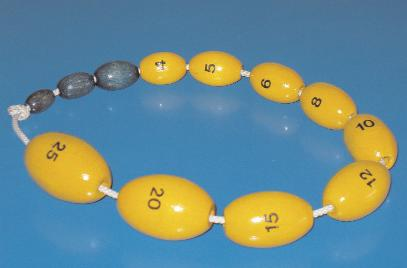
\includegraphics[scale=0.75]{grafici/orchidometro.jpg}
  \end{center}
  \caption{Orchidometro di Prader}
\end{figure}

\begin{figure}[h]
  \begin{center}
	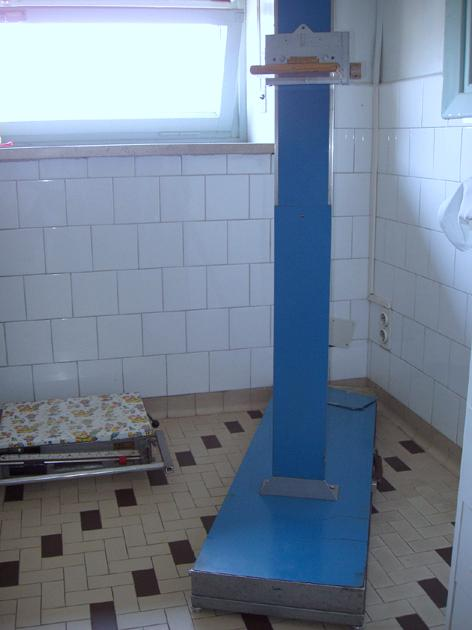
\includegraphics[scale=0.50]{grafici/statimetro.jpg}
  \end{center}
  \caption{Statimetro di Harpenden}
\end{figure}

\subsection{Valutazione ormonale}

\subsection{Analisi statistiche}
